\section{Results and Analysis}

\subsection{Quantitative Results}

The LiDAR-only PointPillars baseline and the MBT-configured detector were
evaluated on the 3,769-sample KITTI validation split. Both experiments used
the same split, classes, point-cloud range, training schedule, effective batch
size, and random seed. The best checkpoint for each model was selected using
overall 3D AP$_{40}$ at moderate difficulty.

\begin{table}[ht]
\centering
\caption{Overall KITTI 3D AP$_{40}$ on the validation split.}
\label{tab:overall_results}
\begin{tabular}{lccc}
\hline
Model & Easy & Moderate & Hard \\
\hline
LiDAR-only PointPillars & 49.5614 & 38.6868 & 36.1066 \\
MBT-configured detector & \textbf{52.1218} & \textbf{41.1813} & \textbf{38.2311} \\
\hline
Difference & +2.5604 & +2.4945 & +2.1245 \\
\hline
\end{tabular}
\end{table}

\begin{table}[ht]
\centering
\caption{Per-class 3D AP$_{40}$ at moderate difficulty.}
\label{tab:per_class_results}
\begin{tabular}{lccc}
\hline
Class & LiDAR-only & MBT-configured & Difference \\
\hline
Pedestrian & 30.3730 & \textbf{32.3544} & +1.9814 \\
Cyclist & \textbf{34.1321} & 33.2382 & -0.8939 \\
Car & 51.5553 & \textbf{57.9512} & +6.3959 \\
\hline
\end{tabular}
\end{table}

The MBT-configured detector improves moderate AP$_{40}$ by 2.4945 points
(6.45\% relative) and improves the overall metric at all three difficulty
levels. The largest moderate-difficulty change is observed for Car
(+6.3959), followed by Pedestrian (+1.9814); Cyclist decreases by 0.8939
points. The LiDAR-only model reaches its best result at epoch 28, whereas the
MBT-configured model reaches its best result at epoch 58. Figure
\ref{fig:validation_convergence} shows all 40 validation measurements.

\begin{figure}[ht]
\centering
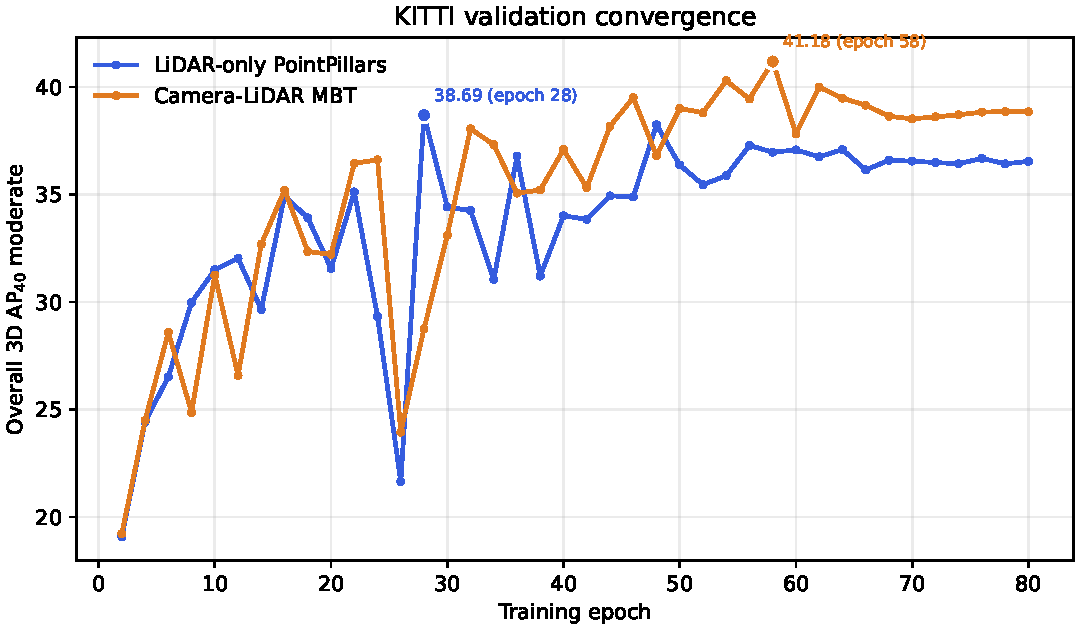
\includegraphics[width=\linewidth]{evaluation_assets/validation_ap40_curve.pdf}
\caption{Overall 3D AP$_{40}$ moderate during training. Validation was
performed every two epochs.}
\label{fig:validation_convergence}
\end{figure}

\subsection{Qualitative Results}

Temporal visualizations were generated on six KITTI Raw drives. Each frame
shows the full 360-degree LiDAR scan, the camera-field-of-view subset supplied
to both models, LiDAR-only predictions, MBT predictions, available tracklet
annotations, and MBT boxes projected onto the camera image. Predictions are
computed independently with no tracking or temporal smoothing. Figure
\ref{fig:qualitative_examples} uses the midpoint frames of three drives chosen
before inspecting their predictions.

\begin{figure}[ht]
\centering
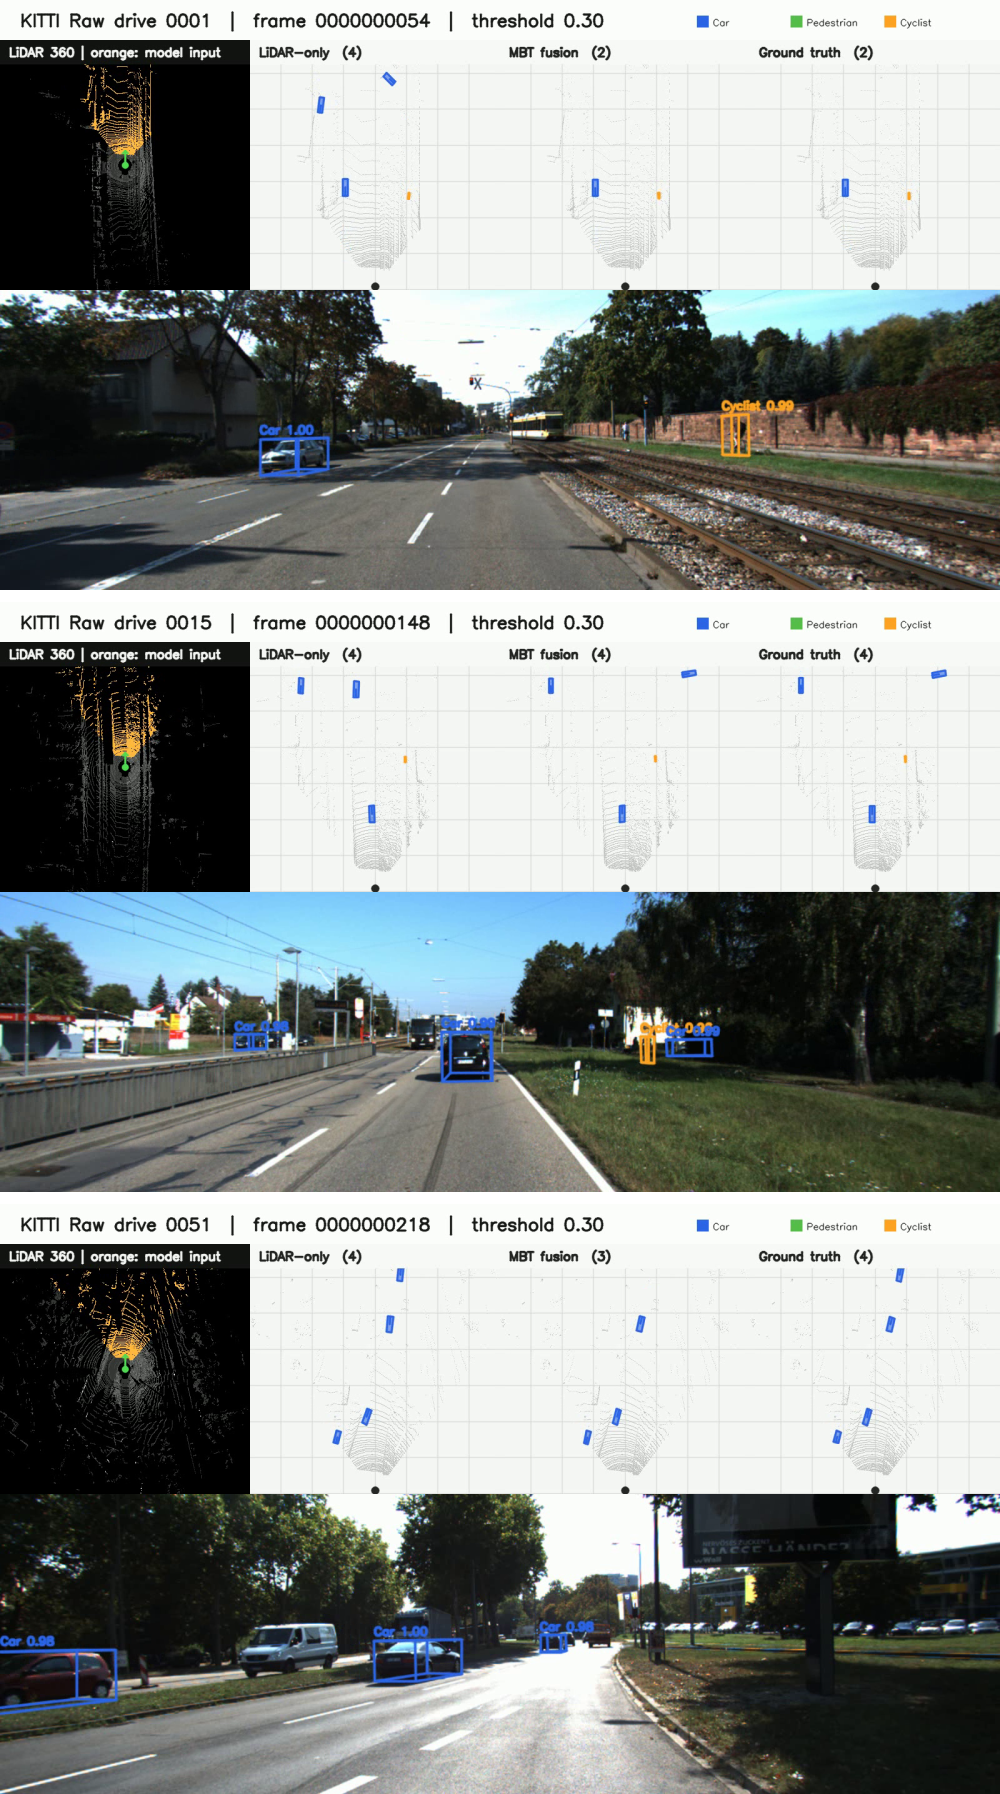
\includegraphics[width=\linewidth]{evaluation_assets/qualitative_midpoint_examples.png}
\caption{Midpoint frames from KITTI Raw drives 0001, 0015, and 0051 at a
display threshold of 0.30. Orange LiDAR points are supplied to the models;
gray points are shown only as a 360-degree reference.}
\label{fig:qualitative_examples}
\end{figure}

These visualizations provide examples of agreement and disagreement between
the two detectors, but they are not an additional AP evaluation. KITTI Raw
tracklets are incomplete, and objects outside the three trained classes may
appear without ground-truth boxes.

\subsection{Camera Ablation}

To test whether the improvement depends on meaningful camera content, the
best MBT checkpoint was reevaluated with normal images, all-black images, and
a deterministic seed-0 derangement of the validation images. The shuffled
condition assigns every LiDAR sample an image from a different validation
sample while leaving its LiDAR points and annotations unchanged.

\begin{table}[ht]
\centering
\caption{Camera-input ablation using the same epoch-58 MBT checkpoint.}
\label{tab:camera_ablation}
\begin{tabular}{lccc}
\hline
Camera input & Easy & Moderate & Hard \\
\hline
Correct image & 52.1218 & 41.1813 & 38.2311 \\
Black image & 52.1218 & 41.1813 & 38.2311 \\
Shuffled image & 52.1216 & 41.1811 & 38.2311 \\
\hline
\end{tabular}
\end{table}

The black-image condition reproduces the normal-image AP$_{40}$ values, and
the shuffled condition changes moderate AP$_{40}$ by only $-0.0002$. Across
17,438 persisted detections, the mean absolute confidence-score change is
$2.08\times10^{-8}$ for black images and $1.83\times10^{-8}$ for shuffled
images; the maximum change is below $3.89\times10^{-5}$ in both cases. Thus,
the evaluated checkpoint is effectively invariant to image content. The
2.4945-point improvement over PointPillars demonstrates a benefit from the
MBT-configured architecture and training, but it cannot be attributed to
meaningful camera--LiDAR fusion. The added LiDAR-side transformer, learned
bottleneck priors, and residual processing are possible sources of the gain.

\subsection{Limitations}

The experiments use one random seed and the KITTI validation split rather
than the official test server, so uncertainty across training runs has not
been measured. The current fusion module does not explicitly align camera
features with the LiDAR BEV geometry, and the camera ablation shows that the
trained checkpoint does not use image content meaningfully. Consequently,
attention-map visualization would not by itself establish multimodal use.
Future work should revise the fusion pathway, repeat the camera ablation after
retraining, and report multiple-seed results. Finally, the temporal figures
use incomplete KITTI Raw tracklets and a fixed display threshold, so they are
qualitative illustrations rather than benchmark measurements.
